\documentclass{beamer}
%USE PDF LATEX to build properly!
\usetheme{progressbar}
\progressbaroptions{titlepage=normal}
\progressbaroptions{headline=sections,frametitle=normal}

\graphicspath{{images/}}

\usepackage[german]{babel}
\usepackage{mathptmx, amsmath}
\usepackage[utf8]{inputenc}
 
\title[]{\textbf{Memory-based exploratory online learning of simple object 
manipulation}\\{\scriptsize Master thesis}}
\author[]{Jan P\"oppel}
\date{05.10.2015}

\begin{document}


\begin{frame}
	\maketitle
\end{frame}

\begin{frame}{Outline}
\tableofcontents
\end{frame}

\section{Task}
\begin{frame}{Scenario}
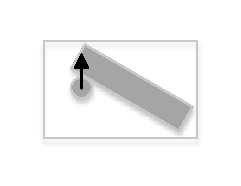
\includegraphics[width=\textwidth]{Scneario.pdf}
\end{frame}

\begin{frame}{Task}
Given an environment and a set of action primitives to control some actuator, incrementally and 
interactively learn a 
\begin{columns}
\begin{column}[c]{.50\textwidth}
\begin{center}
Forward Model
\end{center}

\includegraphics[width=\textwidth]{Forwards} 
\end{column}
\begin{column}[c]{.50\textwidth}
\begin{center}
Inverse Model
\end{center}

\includegraphics[width=\textwidth]{Backwards} 
\end{column}
\end{columns}
\end{frame}

\section{Current Results}
\begin{frame}{Current Results}
Video(s)
\end{frame}

\section{Methods}
\begin{frame}{Methods}
 Created two models \\~\\
\begin{columns}
\begin{column}[t]{.50\textwidth}
Interactions
\begin{itemize}
\item Represent interaction states
\item Split space into subspaces along different interactions
\end{itemize}
\end{column}
\begin{column}[t]{.50\textwidth}
Objects with gate
\begin{itemize}
\item Represent individual object states
\item Introduce gate, distinguishing interaction from no interaction
\end{itemize}
\end{column}
\end{columns}
\end{frame}

\begin{frame}{Method - Interactions}
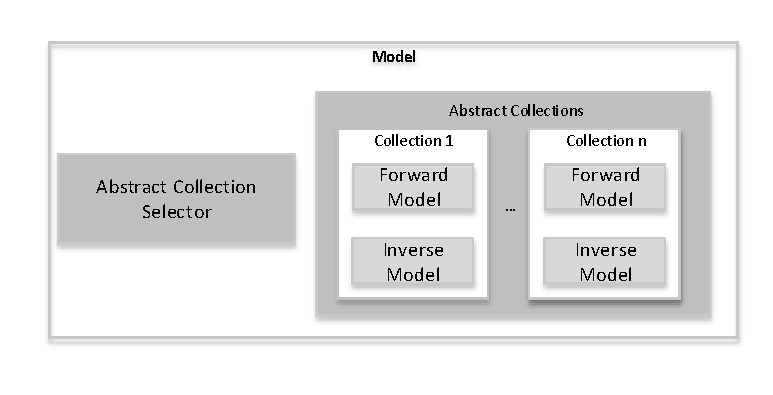
\includegraphics[width=\textwidth]{PairwiseOverview.pdf}
\end{frame}

\begin{frame}{Method - Interactions Prediction}
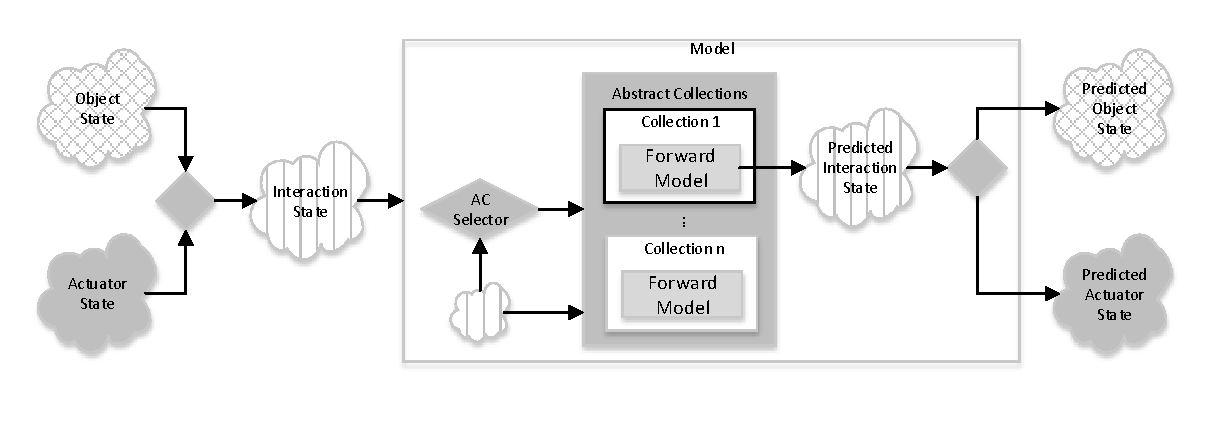
\includegraphics[width=\textwidth]{PairwisePrediction.pdf}
\end{frame}

\begin{frame}{Method - Gate}
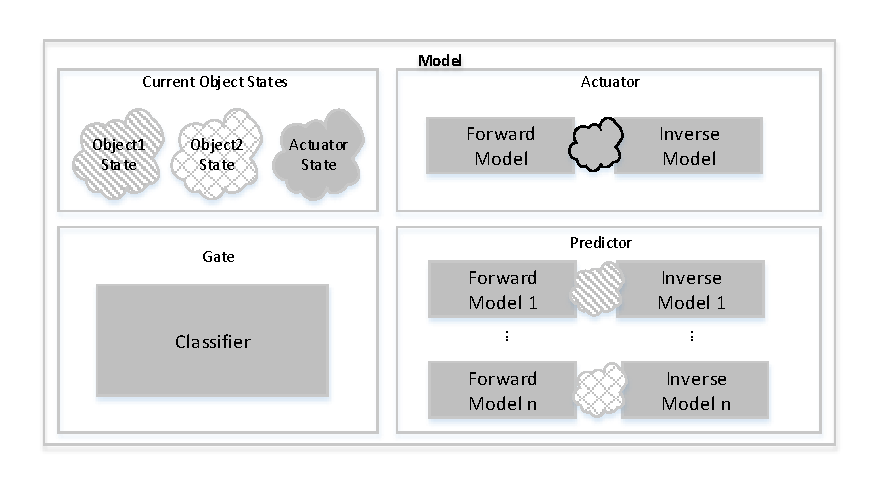
\includegraphics[width=\textwidth]{GateOverview.pdf}
\end{frame}

\begin{frame}{Method - Gate Prediction}
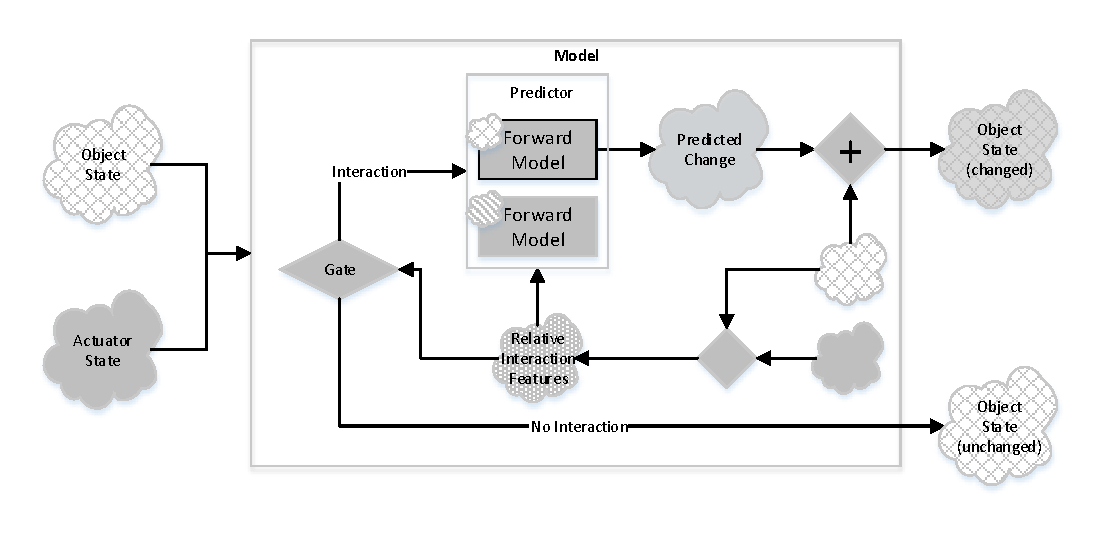
\includegraphics[width=\textwidth]{GatePrediction.pdf}
\end{frame}

\begin{frame}{Method - Gate Planning}
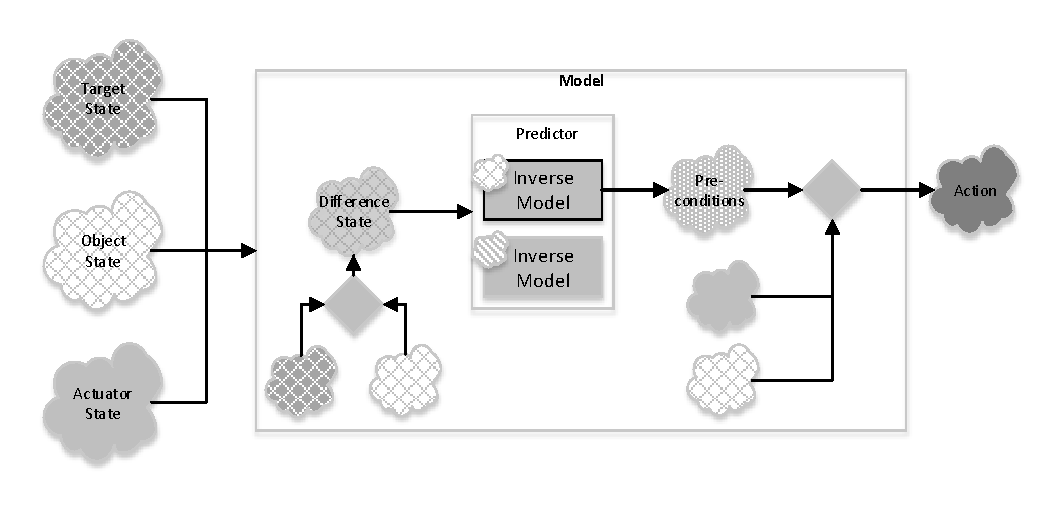
\includegraphics[width=\textwidth]{GatePlanning.pdf}
\end{frame}

\section{Issues}
\begin{frame}{Issues}
\begin{itemize}
\item Incremental update
\item Time constraints for updates and queries due to environment loop
\item Metric problem
\begin{itemize}
	\item Features may have different orders of magnitudes (e.g. orientation/position)
	\item Features may have different importances
\end{itemize}
\end{itemize}
\end{frame}

\section{Technologies}
\begin{frame}{Technologies}
\begin{itemize}
\item Regression and classification models are memory/instance based
\item Adapted the instantaneous topological map (ITM) as main model
\item Developed abstract inverse model to avoid extrapolation and metric problems 
\end{itemize}
\end{frame}

\begin{frame}{Technology - ITM}

\end{frame}

\begin{frame}{Technology - Inverse Model}
Inhalt...
\end{frame}

\section{Evaluation}
\begin{frame}{Evaluation}
Two main tasks in order to test forward and inverse model \\~\\
\begin{columns}
\begin{column}[t]{.50\textwidth}
PushTaskSimulation (Video 1)
\begin{itemize}
\item Train at different starting positions and push the object
\item Use previous prediction as input when testing \\$\rightarrow$ No environment feedback
\end{itemize}
\end{column}
\begin{column}[t]{.50\textwidth}
MoveToTarget (Video 2)
\begin{itemize}
\item Show all feature changes during training
\item Give fixed target position for one object 
\item Operate in open loop $\rightarrow$ Constant environment feedback
\end{itemize}
\end{column}
\end{columns}
\end{frame}

\begin{frame}{Evaluation - PushTaskSimulation}
\begin{itemize}
\item A run is defined as the number of frames until the actuator traveled a certain distance
\item Testruns start at varying starting points
\item Calculate difference to actual object at end of each run
\item Difference defined over keypoints in order to combine position and orientation
\item Test against different number of training runs
\end{itemize}
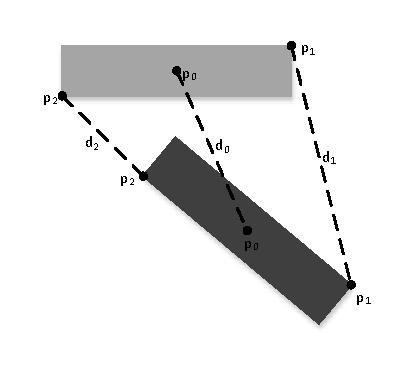
\includegraphics[width=0.45\textwidth]{Keypoints.pdf}
\end{frame}

\begin{frame}{Evaluation - MoveToTarget}
Multiple possibilities
\begin{itemize}
\item Measure number of frames/actions required to reach target
\item Measure distance after fixed number of allowed actions
\item Measure average distance reduction per action
\item Try reduced number of training examples/interactions
\begin{itemize}
	\item e.g. only show position change and no orientation
\end{itemize}
\end{itemize}
\end{frame}

\begin{frame}{Further Evaluations and further features}

\begin{itemize}
\item Evaluate subparts by swapping them out where possible
	\begin{itemize}
	\item E.g. gate classifier/actuator forward model
	\end{itemize}
\item Distinguish testpositions that were not included in trainset and those that are
\item Multiple objects
\item Self-exploration
\end{itemize}
\end{frame}


\begin{frame}
\begin{center}
{\Large Thank you for your attention!}
\end{center}
\end{frame}

\end{document}
